\documentclass[crop,tikz]{standalone}

\begin{document}
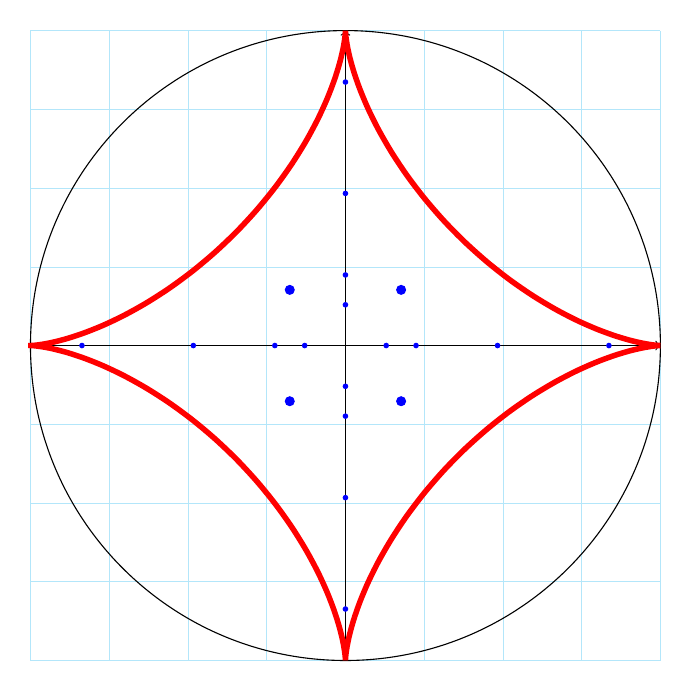
\begin{tikzpicture}
\def\a{1} \def\b{4} \def\scale{1}
\draw[cyan!30,very thin] ({-\b*\scale},{-\b*\scale}) grid ({\b*\scale},{\b*\scale});
\draw[->] ({-\b*\scale},0) -- ({\b*\scale},0);
\draw[->] (0,{-\b*\scale}) -- (0,{\b*\scale});
\draw (0,0) circle ({\b*\scale});
\draw[line width=2pt,red] plot[samples=100,domain=0:\a*360,smooth,variable=\t] ({\scale*((\b-\a)*cos(\t)+\a*cos((\b-\a)*\t/\a)},{\scale*((\b-\a)*sin(\t)-\a*sin((\b-\a)*\t/\a)});

\draw[blue,fill=blue] (0.0,1.9318516525781364) circle (4*0.200000000000000pt);
\draw[blue,fill=blue] (0.0,-0.8965754721680539) circle (4*0.200000000000000pt);
\draw[blue,fill=blue] (0.0,0.8965754721680539) circle (4*0.200000000000000pt);
\draw[blue,fill=blue] (0.8965754721680539,0.0) circle (4*0.200000000000000pt);
\draw[blue,fill=blue] (-0.5176380902050414,0.0) circle (4*0.200000000000000pt);
\draw[blue,fill=blue] (0.0,-0.5176380902050414) circle (4*0.200000000000000pt);
\draw[blue,fill=blue] (0.7071067811865476,-0.7071067811865476) circle (4*0.400000000000000pt);
\draw[blue,fill=blue] (0.5176380902050414,0.0) circle (4*0.200000000000000pt);
\draw[blue,fill=blue] (0.0,-1.9318516525781364) circle (4*0.200000000000000pt);
\draw[blue,fill=blue] (0.7071067811865476,0.7071067811865476) circle (4*0.400000000000000pt);
\draw[blue,fill=blue] (-3.3460652149512318,0.0) circle (4*0.200000000000000pt);
\draw[blue,fill=blue] (0.0,3.3460652149512318) circle (4*0.200000000000000pt);
\draw[blue,fill=blue] (-1.9318516525781364,0.0) circle (4*0.200000000000000pt);
\draw[blue,fill=blue] (0.0,0.5176380902050414) circle (4*0.200000000000000pt);
\draw[blue,fill=blue] (-0.8965754721680539,0.0) circle (4*0.200000000000000pt);
\draw[blue,fill=blue] (-0.7071067811865476,-0.7071067811865476) circle (4*0.400000000000000pt);
\draw[blue,fill=blue] (-0.7071067811865476,0.7071067811865476) circle (4*0.400000000000000pt);
\draw[blue,fill=blue] (3.3460652149512318,0.0) circle (4*0.200000000000000pt);
\draw[blue,fill=blue] (1.9318516525781364,0.0) circle (4*0.200000000000000pt);
\draw[blue,fill=blue] (0.0,-3.3460652149512318) circle (4*0.200000000000000pt);
\end{tikzpicture}

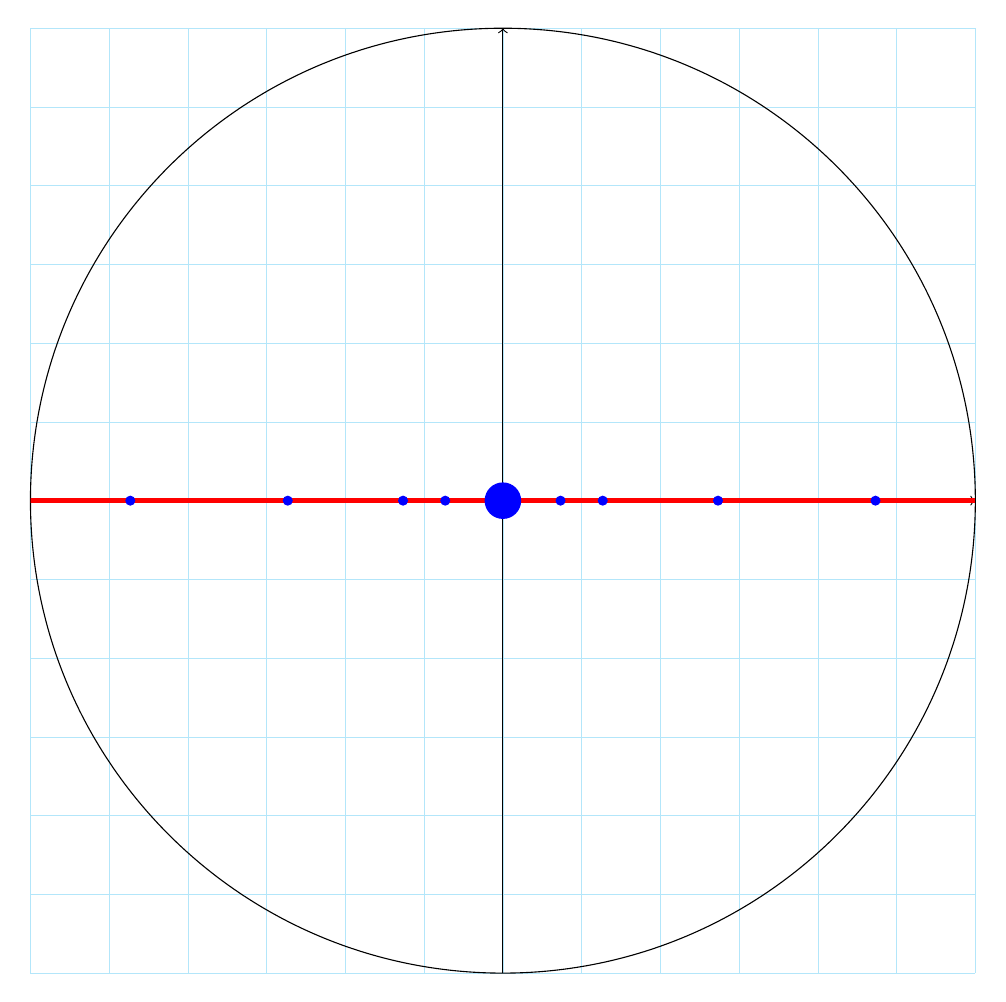
\begin{tikzpicture}
\def\a{1} \def\b{2} \def\scale{3}
\draw[cyan!30,very thin] ({-\b*\scale},{-\b*\scale}) grid ({\b*\scale},{\b*\scale});
\draw[->] ({-\b*\scale},0) -- ({\b*\scale},0);
\draw[->] (0,{-\b*\scale}) -- (0,{\b*\scale});
\draw (0,0) circle ({\b*\scale});
\draw[line width=2pt,red] plot[samples=100,domain=0:\a*360,smooth,variable=\t] ({\scale*((\b-\a)*cos(\t)+\a*cos((\b-\a)*\t/\a)},{\scale*((\b-\a)*sin(\t)-\a*sin((\b-\a)*\t/\a)});

\draw[blue,fill=blue] (-2.732050807568877,0.0) circle (4*0.400000000000000pt);
\draw[blue,fill=blue] (-1.2679491924311228,0.0) circle (4*0.400000000000000pt);
\draw[blue,fill=blue] (1.2679491924311228,0.0) circle (4*0.400000000000000pt);
\draw[blue,fill=blue] (-0.7320508075688772,0.0) circle (4*0.400000000000000pt);
\draw[blue,fill=blue] (0.7320508075688772,0.0) circle (4*0.400000000000000pt);
\draw[blue,fill=blue] (0.0,0.0) circle (4*1.60000000000000pt);
\draw[blue,fill=blue] (4.732050807568877,0.0) circle (4*0.400000000000000pt);
\draw[blue,fill=blue] (-4.732050807568877,0.0) circle (4*0.400000000000000pt);
\draw[blue,fill=blue] (2.732050807568877,0.0) circle (4*0.400000000000000pt);
\end{tikzpicture}

\end{document}